\documentclass[../main.tex]{subfiles}

\begin{document}

\chapter{Introduction}\label{sec:introduction}
The increase of computation and dissemination of computing devices in recent years ($\sim$ 15 years) is undeniable.
Devices with same (or greater) computation power that took the man to the moon is today in a hand's reach and many are used to control machines everywhere.

With this increase on computation power, we can now solve some problems that were not solvable in a reasonable time in the past, thus the \emph{renaissance} of some optimization based methods, such as \todo{Neural networks} and \todo{Artificial Intelligence}.

For other more common methods such \mpc~\cite{GarciaEtAl1989}, this development meant solving more significant problems in less time, sometimes even in real-time~\cite{BesselmannEtAl2008}, and using small computation units smaller than coins~\cite{BanguraMahony2014}.

Consequently the list of possible applications of \mpc{}, increased, instead of using for single equipments in petrochemical plants with large time scales, to control system with scale of districts and cities such as \wdns~\cite{ZhangEtAl2021} and \dhns~\cite{TaylorEtAl2021}.
This presents a gradual insertion of \mpc{} into \cps{}, in which computers and physical machines are tightly coupled.

Nevertheless, for some large-scale systems, the calculation with multiple decision variables may still be expensive.
Needing some subterfuges, such as distributing it into different computation units and making them communicate.
As we will see, this strategy is called \dmpc and come in many flavors.

However, as we will see, not so many studies have been made on the security of the \dmpc{} strategies when units do not communicate honestly.
This work, however, studies what happens when computation units do not work cooperatively in a \dmpc{} framework.

To give a perspective to a general reader on how it can affect the daily life, we tell a simple qualitatively example in form of a story. The conclusion will serve as a main take-away of the possible effects of non-cooperative behaviors.

\section{When greediness backfires}
6 o'clock, on a Christmas morning.
You wake up.
Shivering.
The tips of your fingers are blue and you ask yourself why you accepted to make part of this housing project.

The housing project was set in a undisclosed placed, to test a new sustainable \dhn{}.
Engineers from all around the world were invited to take part of a project for a duration of one year, to test drive the \dhn{} and file bugs.

Nourishment and all other amenities would be payed.
So you willingly accepted.
What could go wrong?

It seemed okay-ish until $6$ weeks ago, when the days became shorter and shorter and the temperatures colder and colder.

You climb out of the bed and take a look at the central temperature control indicator of your house.

The outside temperature is 2$^{o}$C and the mean temperature inside is 5$^{o}$C.
The control indicator is on, but there is a flashing orange LED panel indicating

\begin{quote}
  CONSENSUS NOT REACHED
\end{quote}

Something is wrong.
This is the first time since you arrived you see this message.
And there is less than one week to finish the project.

You take your coat and look outside your window, you observe the central distributing unit, in the middle of the \emph{cul-de-sac} you live.
A similar orange light is flashing.

You go outside to see if there is anything you can do.

Apparently, engineers think alike and all of your neighbors are gathered.



After showing the indubitable proofs, he finally breaks down and tells the truth.



discovered


%   \begin{figure}[H]
%     \centering
%     
\includegraphics[The tips of your.75\textwidth]{../img/district_3d_cycles.png}
% % ./docstheseplot -o ../../docs/img/quantiteAvecTriche4 -i  ../../data/matlab/tricheQuantite/dmpcQuantity4systemsTriche_.mat --quantiteAvecTriche4
%     \caption{A Cul-de-sac with 4 houses}\label{fig:culdesac}
%   \end{figure}




\begin{example}[Effects of a malicious agent]\label{ex:qualitative_example}
  Imagine we have a large system whose overall objective (cost, comfort etc) we want to optimize, but its sub-parts are coupled.
  To solve this problem, a number of \emph{agents interact}.

  In the decomposition used in this work the agents need to exchange values with another agent which referees what we call a \emph{negotiation}. This referee we call \emph{coordinator}.
  The coordinator sends all agents a message, personalized for each agent, which we will call $\theta_{i}$. The indices $i$ indicate the number of the agent.
  In return, each agent responds the coordinator by sending a message, which we will call $\lambda_{i}$.
  This message $\lambda_{i}$ usually depends on the message $\theta_{i}$.\\
  We can see a scheme of the exchanges in Fig.~\ref{fig:ex_exchange_agents}

  % \pagebreak

  % \begin{minipage}[t]{1.0\linewidth}
  %   \vspace{.25cm}
  % \end{minipage}
  \begin{figure}[H]
    \centering
    \begin{tikzpicture}[font=\small,thick,node distance=3*0.6180cm and 0.6180cm,every node/.style=rectangle,
      mpcSmall/.style={fill=mpc_agent, minimum height=0.6180*2cm, minimum width=2cm},
      coordinator/.style={fill=mpc_coordinator, minimum height=0.6180*3cm, minimum width=6cm},
      ]

      \node[draw, mpcSmall,] (block1) {\small Agent 1};
      \node[fill=none, draw=none, right=of block1,] (mult) {\bf $\dots$};
      \node[draw, mpcSmall, fill=mpc_agent, right=of mult,] (blockM) {\small Agent M};
      \node[draw, coordinator, below=of mult,] (coordinator) {Coordinator};

      \draw[-latex,line width=1pt,red] (block1.south)+(0.4,.0) -- ( coordinator.north -| {$(block1.south)+(0.4,.0)$}) node [right,midway] {$\lambda_{1}$\ \faUserSecret};
      \draw[latex-,line width=1pt] (block1.south)+(-0.4,0) -- (  coordinator.north -| {$(block1.south)+(-0.4,0)$}) node [left,midway] {$\theta_{1}$};
      \draw[-latex,line width=1pt] (blockM.south)+(0.4,.0) -- ( coordinator.north -| {$(blockM.south)+(0.4,.0)$}) node [right,midway] {$\lambda_{M}$};
      \draw[latex-,line width=1pt] (blockM.south)+(-0.4,0) -- (  coordinator.north -| {$(blockM.south)+(-0.4,0)$}) node [left,midway] {$\theta_{M}$};
    \end{tikzpicture}
    \caption{Exchange between agents and coordinator.}\label{fig:ex_exchange_agents}
  \end{figure}
  Observe in Fig.~\ref{fig:ex_exchange_agents} that agent 1 sends a suspicious $\lambda_{1}$. Instead of sending the message it was supposed to send, it modifies it before sending to the coordinator.
  This can be considered as a \fdi{} attack, as we will see later (\S\ref{sec:anomalous}).

In this example we have a system with $4$ agents and a coordinator. The objective is to minimize a given function $J$. While all other agents work cooperatively, agent 1 is ill-intentioned. In Fig.~\ref{fig:change_in_j}, we can see the effects of changes in the $\lambda_{1}$ sent on the objectives of each agent $J_{i}$ and the overall objective $J^{\star}$ (in blue).
  \begin{figure}[H]
    \centering
    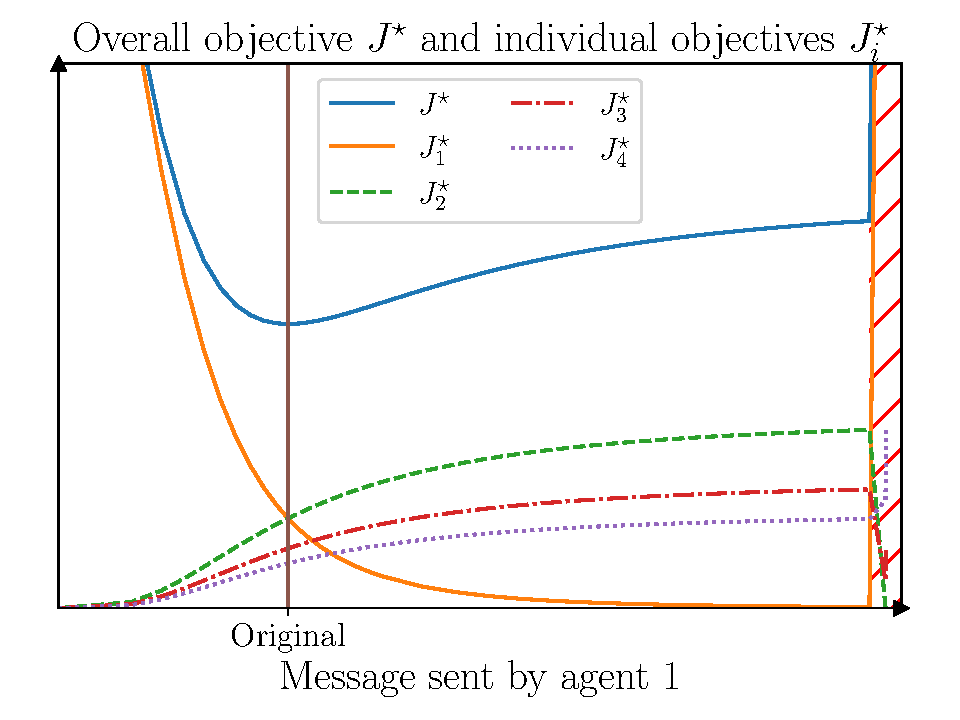
\includegraphics[width=.5\textwidth]{../img/qualitative_example.pdf}
% ./docstheseplot -o ../../docs/img/quantiteAvecTriche4 -i  ../../data/matlab/tricheQuantite/dmpcQuantity4systemsTriche_.mat --quantiteAvecTriche4
    \caption{Changes in objectives depending on message sent by agent 1.}\label{fig:change_in_j}
  \end{figure}
  Observe that the blue curve has its minimum value only when the $\lambda_{1}$ is the original one, every other message makes the resulting system sub-optimal.

  On the other hand we can see that agent 1 can manipulate the negotiation so it can privileged itself (orange curve) at the expense of all others (green, red and purpler curves). This selfish behavior can even destabilize the system, represented by the red hatched area on the graph.
\end{example}

\section{Motivation and Contributions}

\todo{Things to say here:
  \begin{itemize}
    \item \cps{} are systems in which computers and physical machines are tightly coupled.
    \item Increase of large-scale problems Nowadays problems (some examples)
    \item Security problems in those systems \\Here I can give some examples such as Stuxnet \cite{Langner2011}, Brazil blackouts in 2010 \cite{Conti2010}, Ukraine Power System Attack and other attacks (use examples in~\cite{DingEtAl2018,Bindra2017})%
  \end{itemize}
  maybe use https://csiac.org/articles/security-of-cyber-physical-systems/??
}

\cite{DibajiEtAl2019}
A more bibliometric approach with trends in control can be seen in~\cite{ZacchiaEtAl2019}.


From example~\ref{ex:qualitative_example}, we can see the two main effects of a attack: Loss of optimality and eventually breakdown of the control strategy.

While one of them can sometimes be acceptable (depending on the suboptimality), the other is absolutely inadmissible, principally when we are talking about \cps{} that are essential, like electricity and water supply for instance.

So, our goal is to reduce those effects as much as possible.
And to guide us on the quest to minimize them, we can raise some questions:

\simplebox{
  \begin{itemize} \bfseries
    \item Can we detect the attack?
    \item Can we identify the ill-intentioned agent(s)?
    \item Can we mitigate the effects of the attack?
  \end{itemize}
}
This work has as objective to answer these questions, at least for specific cases which will be formally presented.

To understand and answer those questions, we divide this work into two parts.

\paragraph{Part~\ref{part:mpc_intro}} It serves as a gentle introduction to \dmpc{} and attacks.

For a unfamiliar reader, Chapter~\ref{sec:decomposing_mpc} explains what is a \mpc{} to begin with and shows some of the challenges to decompose it.
Chapter~\ref{sec:topology_trust} discuss possible topologies used for those decompositions.
In Chapter~\ref{sec:anomalous} we define anomalous behaviors, give some examples, we categorize them and present some methods used in the literature to prevent and combat them.

\paragraph{Part~\ref{part:safe_dmpc}} It contains the contributions of this work.

Chapter~\ref{sec:primal_decomposition} presents the decomposition studied in this work (primal decomposition), some of its vulnerabilities and how they can affect the performance of the system (here we take up Example~\ref{ex:qualitative_example} giving it a more quantitative approach).
Once we know the vulnerabilities and possible effects of attacks, we divide the mitigation problem into manageable parts.
\\ First in Chapter~\ref{sec:safe_pddmpc_eq}, we analyze an unsophisticated problem, so we can assess the difficulties that can be found when solving the mitigation problem. From the analysis of the problem we propose a detection and mitigation mechanism, followed by an academical example to illustrate.
\\Then, in Chapter~\ref{sec:safe_pddmpc_ineq}, we analyze a similar problem but with a twist. As we will see, just one small modification on the initial problem can increase exponentially its complexity.
From the analysis of the newly-found problem we propose a similar strategy, but with adequate modifications to contain the exponential nature of the problem.
\todo{\\Finally, we continue in Chapter~\ref{sec:safe_pddmpc_ineq_reconst} the methodology and explore some more properties to create a less conservative strategy.}
\\Then, we conclude this work in Chapter~\ref{sec:conclusion} with a discussion about the results found during this study, benefits as well as shortcomings. Some of this discussion leads to open questions which can incite new works.

% Since those questions are still open, this work has as objective to discuss these questions by analyzing the recent literature and schematizing the security in decomposition methods for Model Predictive Control passing by the following items:
% \begin{itemize}[label=$\bullet$]
%   \item decomposition methods;
%   \item topology;
%   \item points of vulnerability;
%   \item how malicious agents can benefit from such vulnerabilities;
%   \item effects on the overall system;
%   \item possible ways to mitigate.
% \end{itemize}
% We use some conclusions of the discussion to develop safe algorithms for a \dmpc\ framework.

\section{Publications}
The work and discussion presented in this thesis yielded the following publications
\begin{itemize}
  \item Published
        \begin{description}
          \item[\cite{NogueiraEtAl2021}] Conference article for the SysTol'21
          \item[\cite{NogueiraEtAl2022}] \todo[correct citation]{} Conference article for the NecSys'22
        \end{description}
  \item Under Review
  \item In Preparation
\end{itemize}



% \chapterEndOrnament

\end{document}
